\documentclass[tikz,border=2pt]{standalone}
\renewcommand{\familydefault}{\sfdefault}
\usetikzlibrary{arrows.meta,calc,positioning}
\tikzset{every picture/.style={line width=1pt, >=Stealth},
         hl/.style={fill=black, fill opacity=0.12, text opacity=1}}
\begin{document}
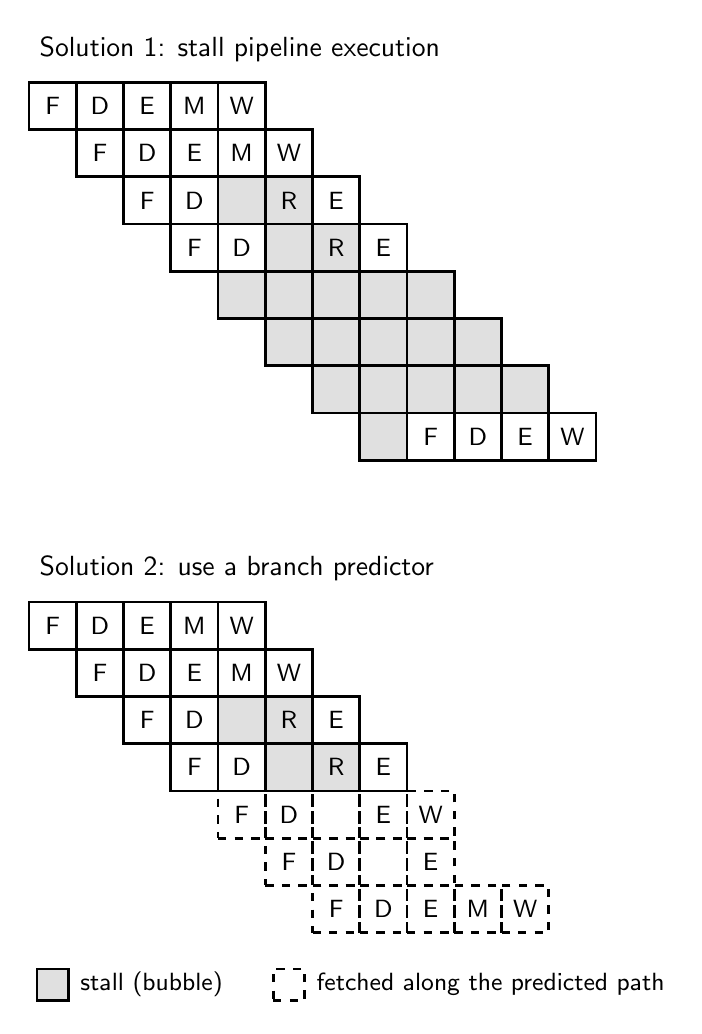
\begin{tikzpicture}[x=0.6cm, y=0.6cm, cell/.style={draw, minimum size=0.6cm, font=\small},
    stall/.style={hl}, predicted/.style={dashed}]
  % \pipe{row}{first cycle}{stage/style, ...}: one instruction, one cell per clock cycle
  \newcommand{\pipe}[3]{\foreach \v/\s [count=\i from 0] in {#3} \node[cell, \s] at (#2 + \i, -#1) {\v};}
  \node[anchor=west] at (-0.5, 1.2) {Solution 1: stall pipeline execution};
  \pipe{0}{0}{F/, D/, E/, M/, W/}
  \pipe{1}{1}{F/, D/, E/, M/, W/}
  \pipe{2}{2}{F/, D/, /stall, R/stall, E/}
  \pipe{3}{3}{F/, D/, /stall, R/stall, E/}
  \pipe{4}{4}{/stall, /stall, /stall, /stall, /stall}
  \pipe{5}{5}{/stall, /stall, /stall, /stall, /stall}
  \pipe{6}{6}{/stall, /stall, /stall, /stall, /stall}
  \pipe{7}{7}{/stall, F/, D/, E/, W/}
  \begin{scope}[yshift=-6.6cm]
    \node[anchor=west] at (-0.5, 1.2) {Solution 2: use a branch predictor};
  \pipe{0}{0}{F/, D/, E/, M/, W/}
    \pipe{1}{1}{F/, D/, E/, M/, W/}
    \pipe{2}{2}{F/, D/, /stall, R/stall, E/}
    \pipe{3}{3}{F/, D/, /stall, R/stall, E/}
    \pipe{4}{4}{F/predicted, D/predicted, /predicted, E/predicted, W/predicted}
    \pipe{5}{5}{F/predicted, D/predicted, /predicted, E/predicted}
    \pipe{6}{6}{F/predicted, D/predicted, E/predicted, M/predicted, W/predicted}
  \end{scope}
  \node[cell, stall, minimum size=0.4cm, label=right:{\small stall (bubble)}] at (0, -18.6) {};
  \node[cell, predicted, minimum size=0.4cm, label=right:{\small fetched along the predicted path}] at (5, -18.6) {};
\end{tikzpicture}
\end{document}
